\section{G Scintillator Geometry and Light guides }

When a particle is passing through the scintillator, it ionizes the material and generates scintillation light. These photons travel via different paths through the scintillator, can be absorbed and reflected, then get converted by the photocathode of the Photomultiplier Tube (PMT), generating a photoelectron current. This current is amplified by the PMT and becomes a measurable electronic pulse (see Fig: (pulse) in time walk or shielding section). Finally, the pulse passes through the electronic system and is read out by the computer. All these various processes affect the total time resolution $\sigma_{ToF}$. Therefore, it is convenient to parameterize the length averaged time resolution $\overline{\sigma_{ToF}}$ by
\begin{equation}
\overline{\sigma_{ToF}}=\sqrt{\sigma_{0}^{2}+\frac{\sigma_{1}^{2}+(\sigma_{p}\frac{L}{2})^{2}}{N_{pe}exp(-\frac{L}{2\lambda})}} .
\label{eq:1}
\end{equation}
The parameters in this equation quantify the characteristics of the detector geometry and components, here, $\sigma_{0}$ is the intrinsic resolution of the electronics and other processes that are independent of the light intensity, $\sigma_{1}$ models the jitter in the combined single-photoelectron response of the scintillator and PMT, and $\sigma_{P}$ accounts for path length variations in the light collection. The distance from the source to the PMT, which for $\overline{\sigma_{ToF}}$ is taken to be half the length of the counter($\frac{L}{2}$), and $\lambda$ is the attenuation length of the scintillator. $N_{pe}$ is the average number of the photoelectrons seen by the PMT of a counter with an infinitely long attenuation length. The statistical behavior of $\sigma_{1}$ and $\sigma_{p}$ is encoded by scaling the single-photoelectron responses by $\sqrt{N_{pe}}$.

The geometry of the individual FToF12 detectors has to be optimized, since it influences the time resolution. Figure~\ref{f:averagesigma} uses equation~\ref{eq:1} to show how the length, width, and thickness of detectors typical for the CLAS12 design requirement affect the time resolution, where he parameters of the time resolution for the existing panel 1a counters are given in Ref ~\cite{smith1999time}. The design requirement for panel 1b is to achieve a combined time resolution for panel 1a and 1b of $80\;ps$ for all scintillator up to $4\;cm$ length.
\begin{figure}[ht!]
\centerline{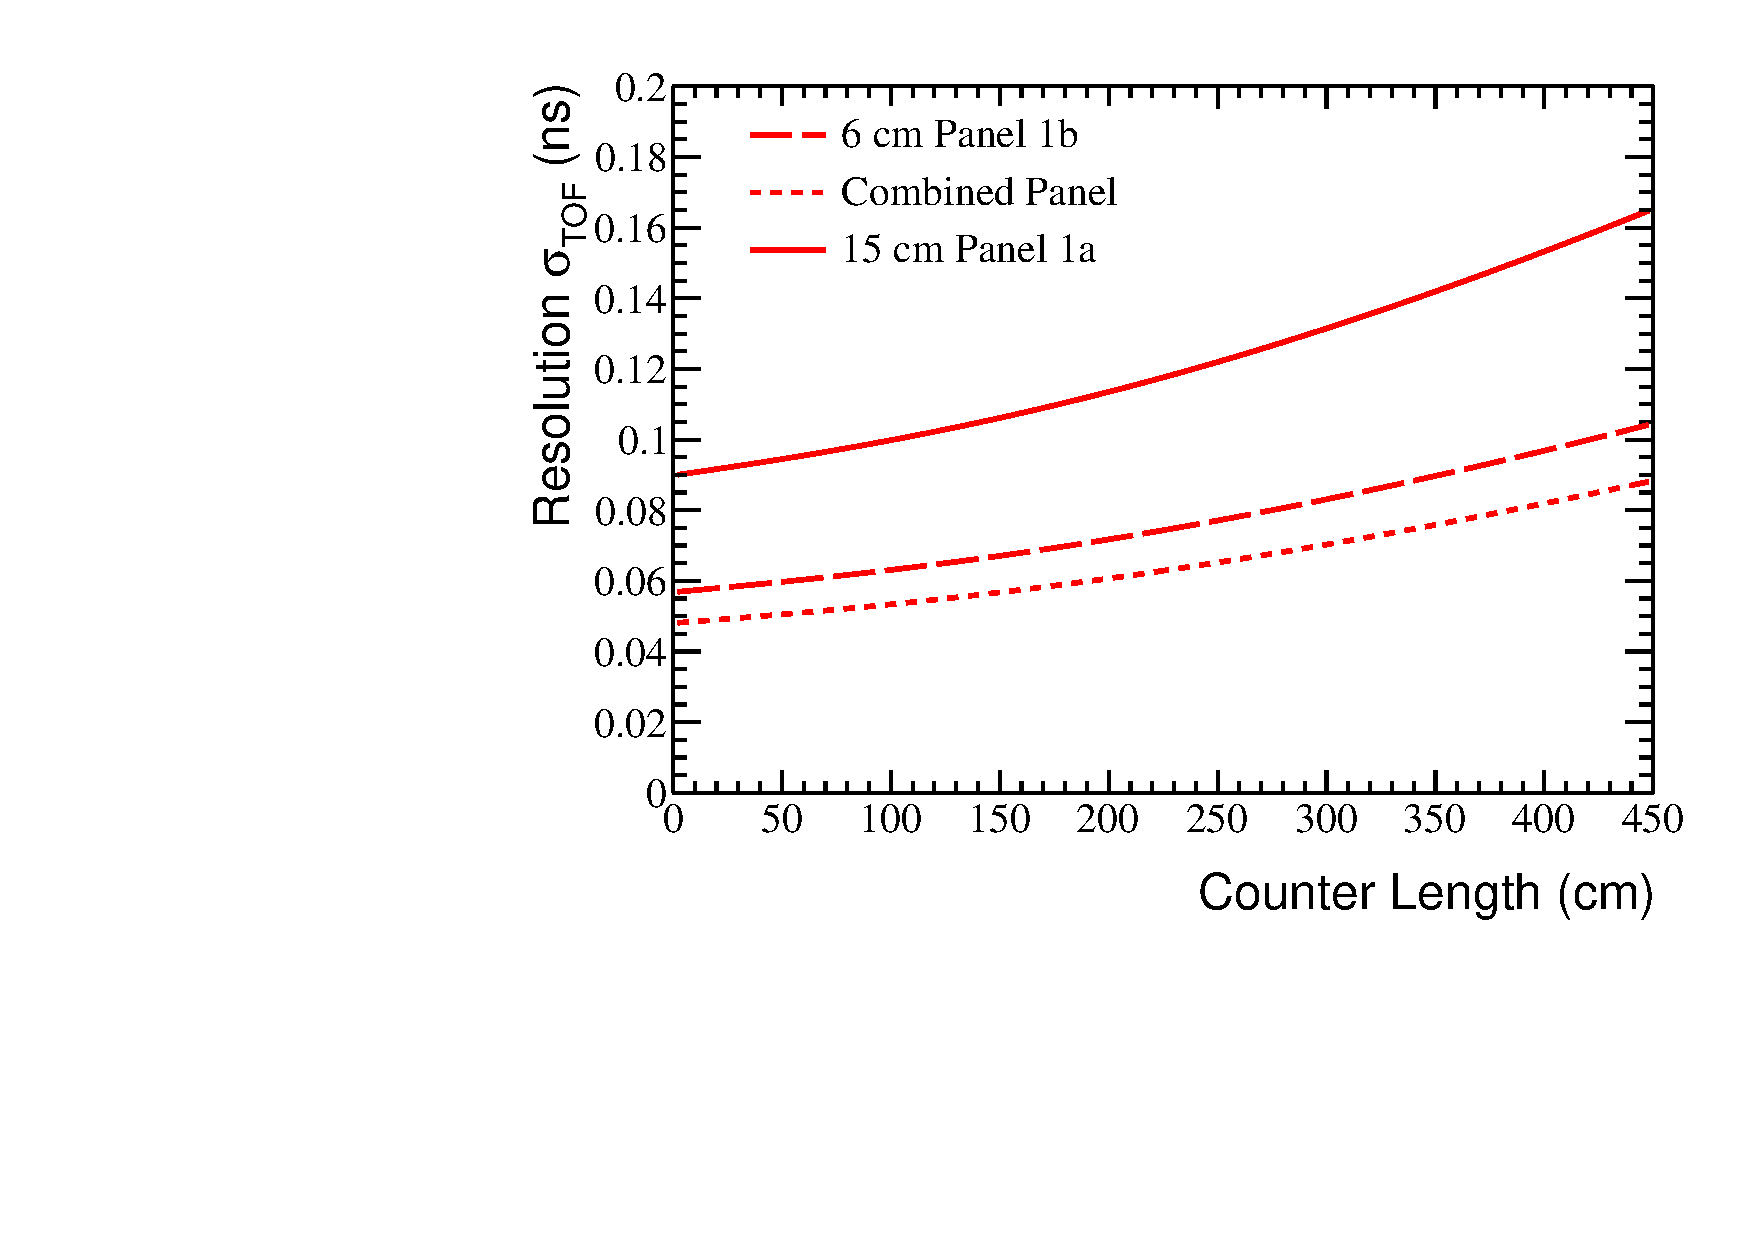
\includegraphics[width=13cm,height=10cm]{ye/fig_ye_geometry/DR.pdf}}
\caption{Solid line, the measured and parameterized average standard deviation $\overline{\sigma_{ToF}}$ time resolution of the existing panel-1a counters ($15\;cm$ wide, $5\;cm$ thick) fit with an assumed intrinsic electronic resolution of 40 ps ~\cite{smith1999time}. Scaling the parametrization by $\sqrt{\frac{2}{5}}$ leads to the  Long dashed line representing the new panel-1b counters (6cm wide, 6cm thick) and short dashed line the combined panel-1a and panel-1b counters time resolution.}
\label{f:averagesigma}
\end{figure}

The most obvious improvement of the time resolution of a detector can be accommodated by increasing the photon statics $N _{pe}$, since the time resolution is proportional to $\sqrt{N_{pe}}$. The number of photons reaching the photocathode scales with the ratio of PMT entrance over exit window areas and the thickness of the scintillator. Given the same PMT diameters, changing the geometry (width $\times$ thickness) from $15\times5\;cm^{2}$ to $6\times6\;cm^{2}$ leads to an increase of $N _{pe}$ by $\frac{15}{6}$. The loss of light from a scintillator can occur in two basic ways; one is the escape of light at the scintillator surface. The simplest and most common practice is to redirect escaping light by total reflection. To maximize the internal reflection, any reflecting film should be loosely wrapped with an air gap to the scintillator, which is described in Sec.I. The other one is through absorption by the scintillation material itself, which is related to the attenuation length consideration described in Set.H.

In contrast to the total reflection requirement discussed above, for the coupling between the scintillator and the PMT, the refraction index change should be minimized to maximize light transmission. Additionally, the PMT is often coupled to the scintillator by a light guide to match the geometry of scintillator to the circular entrance surface of PMT, as in the case of the FToF panel 1a detectors. In the prototyping phase, simulations done to optimized the shape and length of light guides coupling the square exit window of the scintillator to the circular PMT entrance window were carried out. Under best conditions a monotonically increasing a mount of light is lost up to a light guide length of $6\;cm$, which would already liit the over all acceptance of the CLAS12 detectors. Hence the simulation shows that the best light transmission is achieved when the PMT is directly attached to the scintillator. The result was experimentally verified by comparing the scintillator without and with 7cm-long light guide. In order to quantify the time resolution with or without light guide, three-bar time resolution measurements described in Sec. III B were utilized to extract the time resolution of the middle bar under both conditions, respectively. Without light guides, the Hamamatsu PMTs were directly mounted to the left and right ends of a $5 \times 5 \times 150\;cm^{3}$ BC408 scintillator. With light guides, the light guides were first wrapped with aluminized mylar and then
attached to both ends of the same $5 \times 5 \times 150\;cm^{3}$ BC408 scintillator, and the same Hamamatsu PMTs were mounted to light guides.
\begin{figure}[ht!]
\centerline{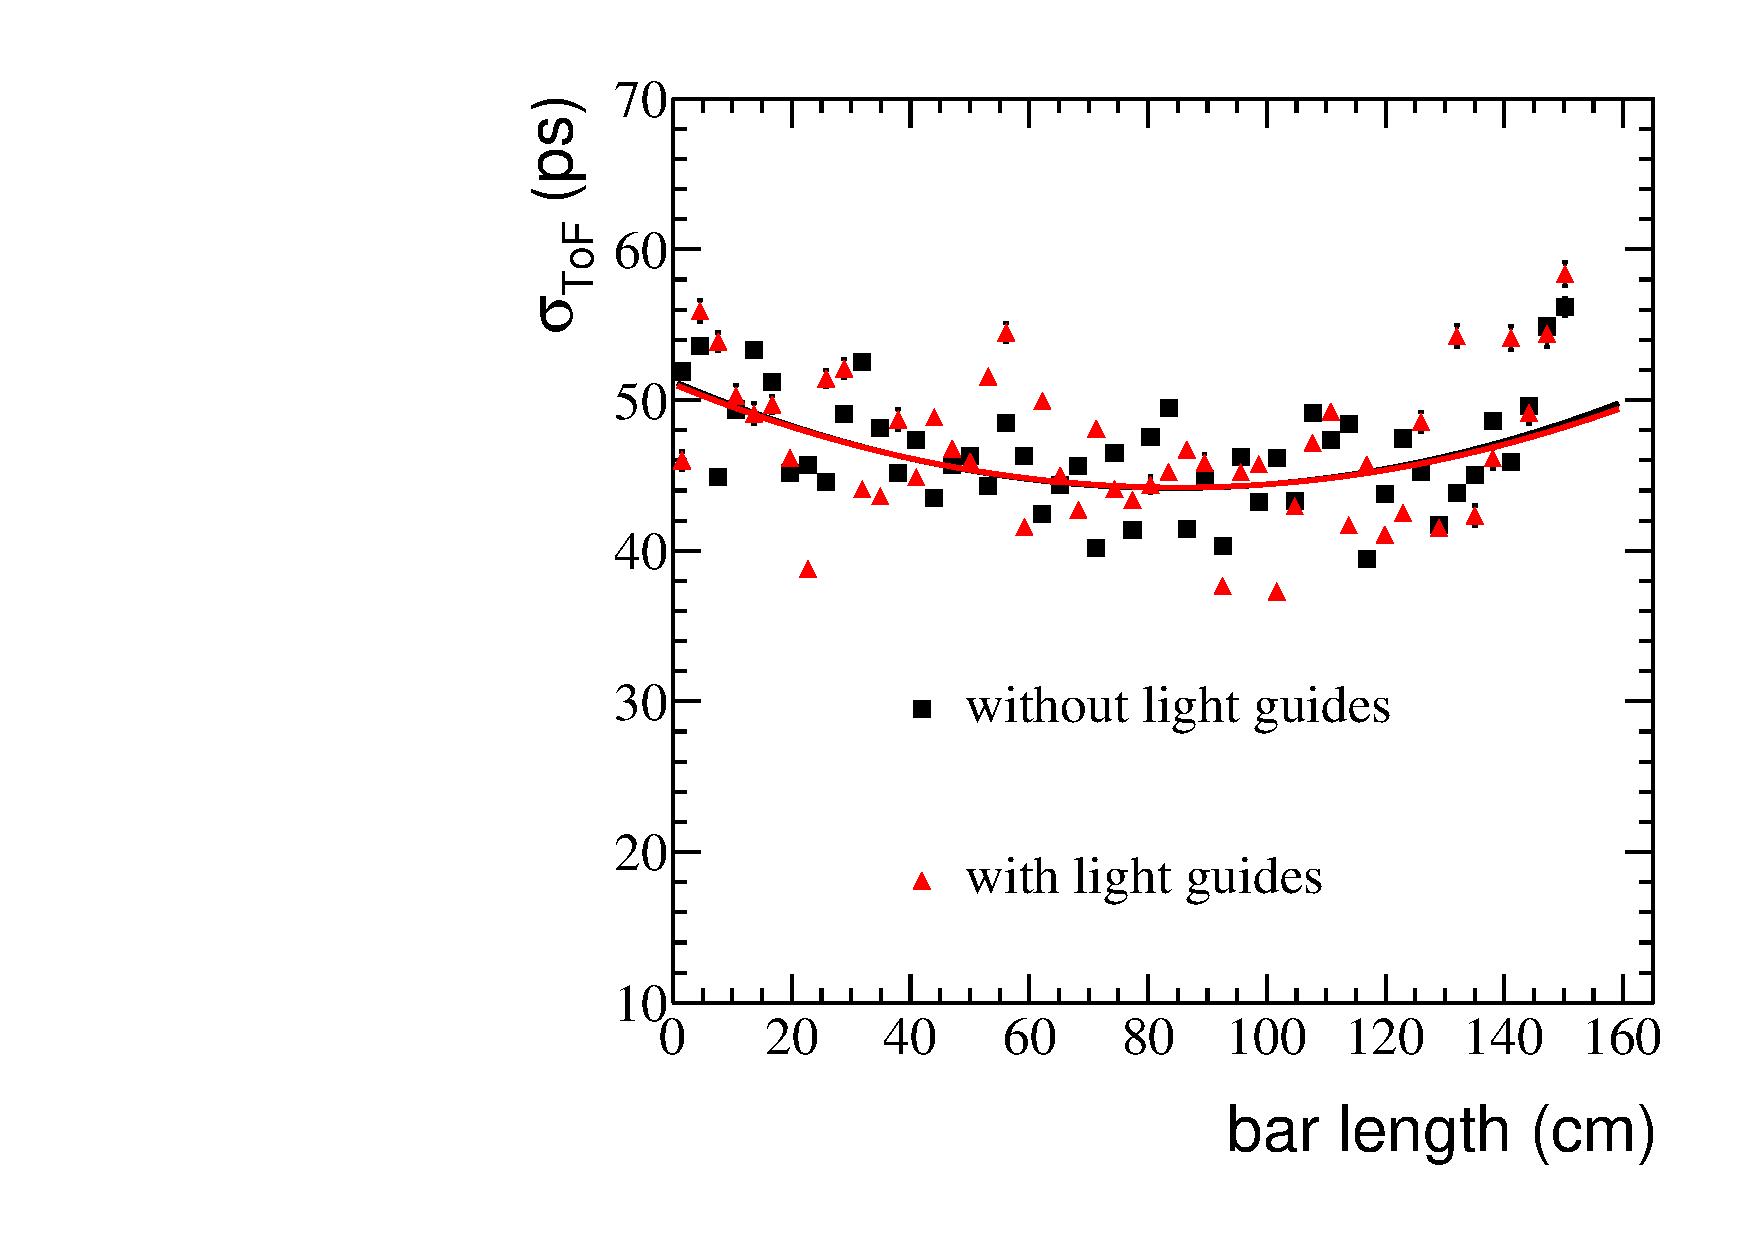
\includegraphics[width=15cm,height=12cm]{ye/fig_ye_geometry/TR_LG.pdf}}
\caption{Black squares, position dependent time resolution of a $5 \times 5 \times 150\;cm^{3}$ BC408 scintillator with and red triangles without light guides. }
\label{f:lightguides}
\end{figure}
Figure~\ref{f:lightguides} shows that the average time resolutions of scintillator with and without light guides are $46.879\;ps$ and $46.519\;ps$, respectively. Even though, the time resolution of scintillator without light guide is a slightly better, the influence of the light guide is still negtigible with in error bars, eliminating the light guides allows for long scintillators covering full fiducial region of CLAS12.
